%--------------------------------------
% Spécifications du chat Felix - Camix
%
% CU
%--------------------------------------

\section{Cas d'utilisation}
\label{sec:cu}

La figure~\ref{sec:cu:figcu} présente les cas d'utilisation du chat.

\medskip
\begin{figure}[h!]
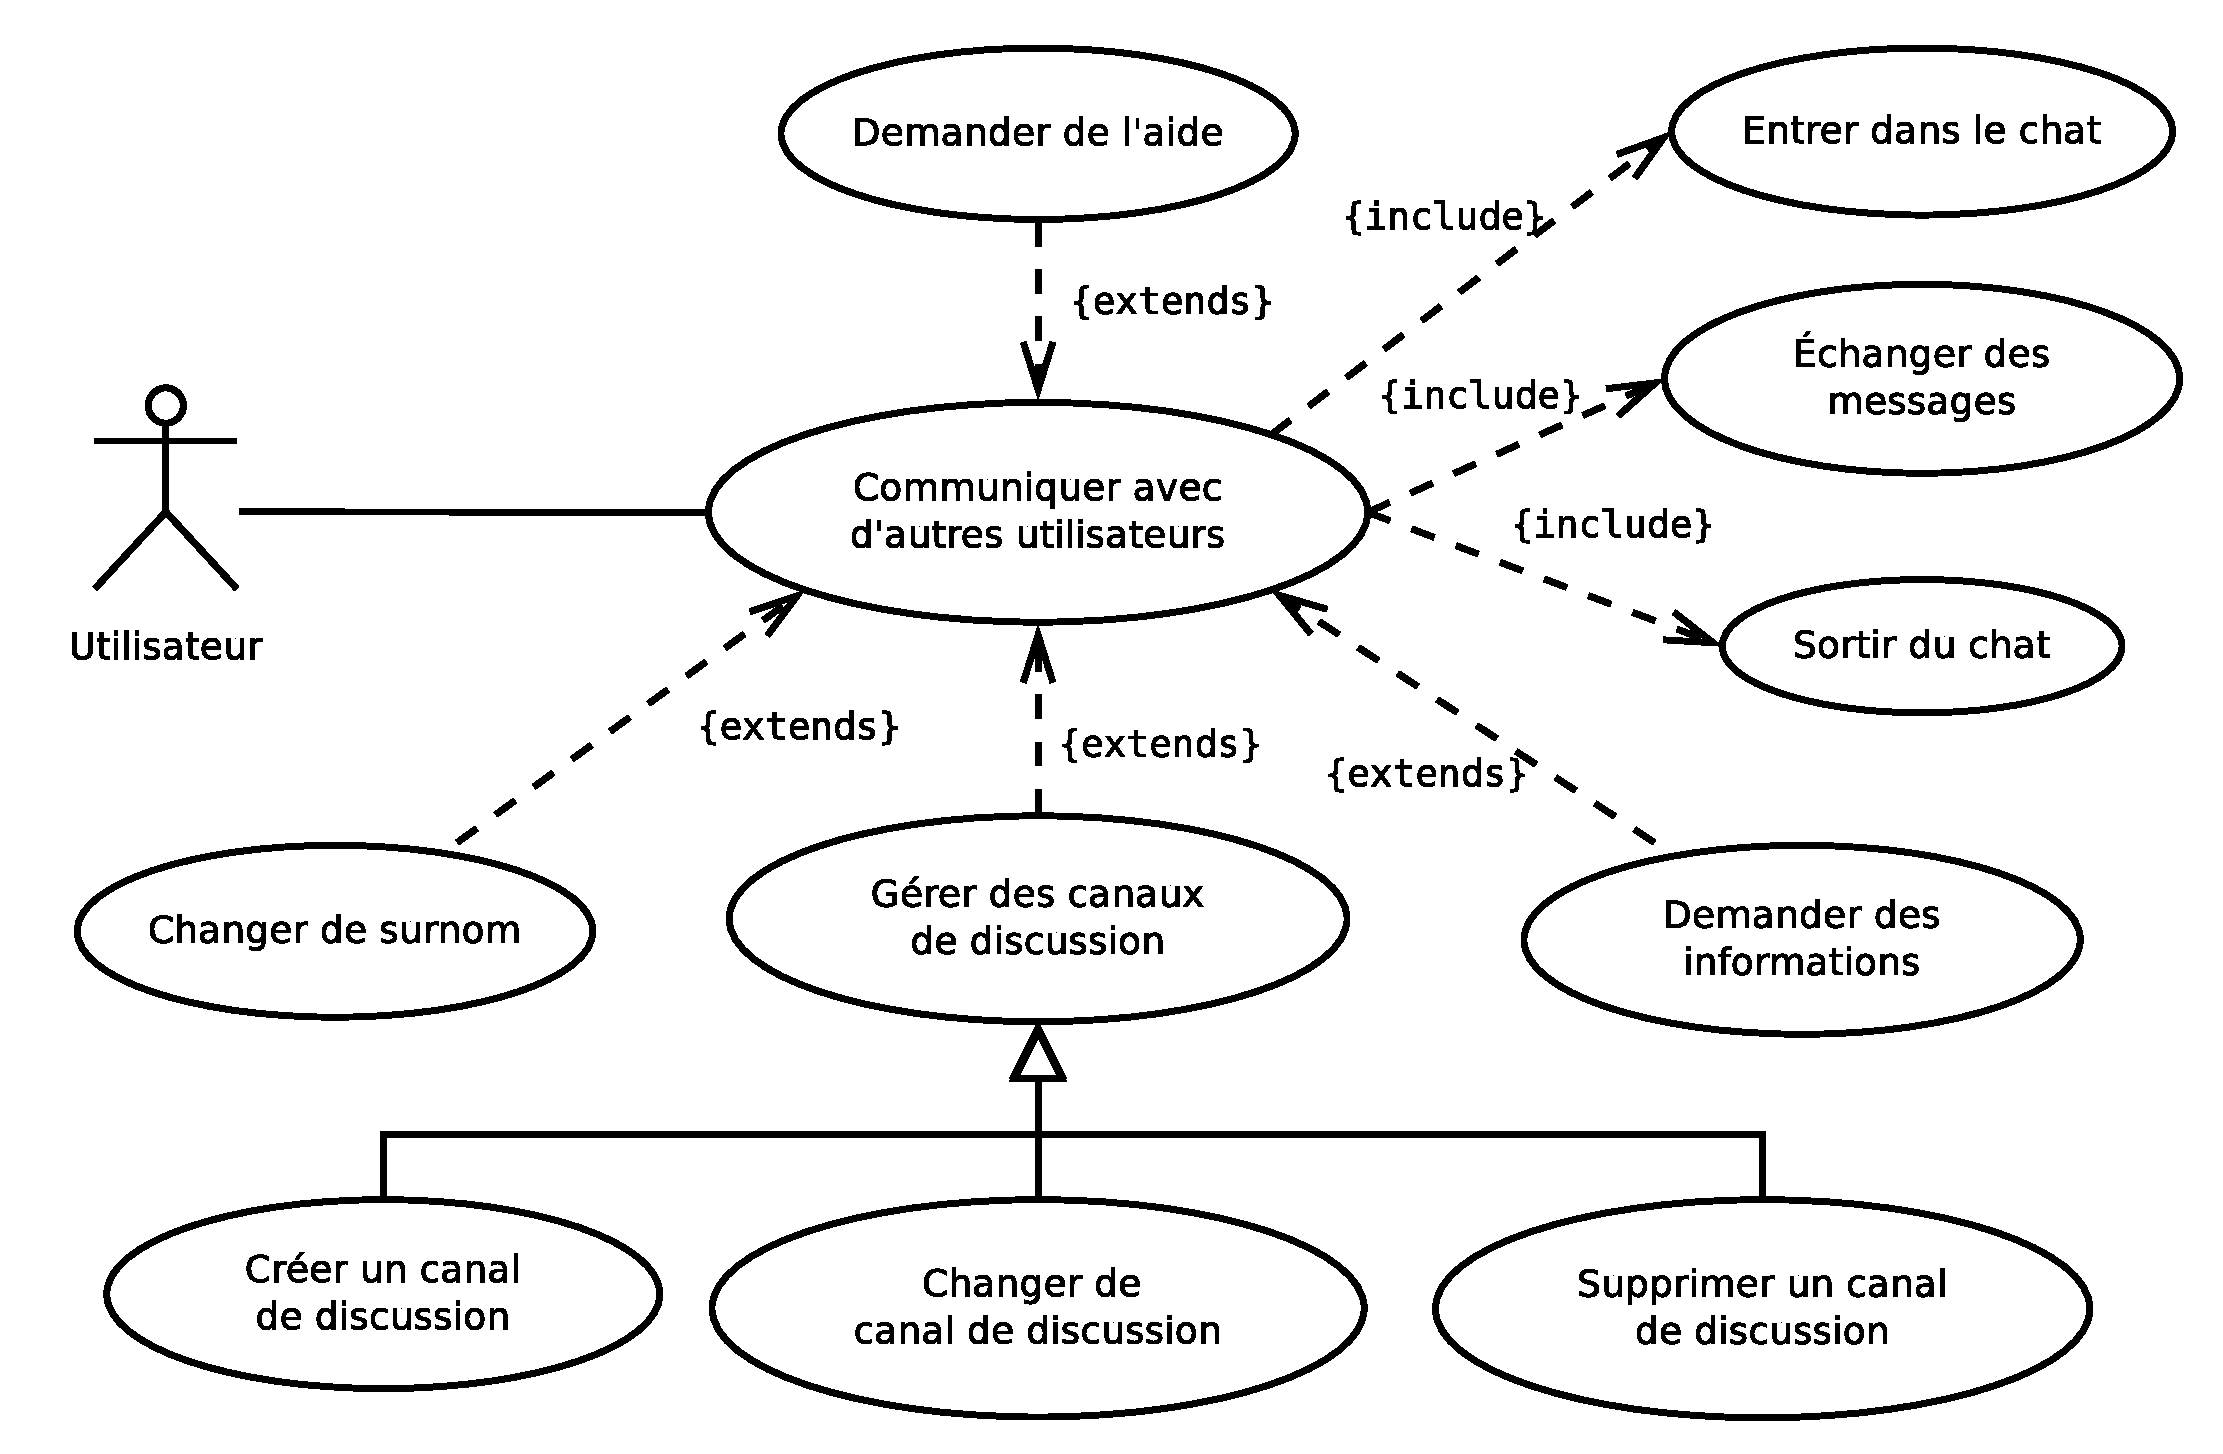
\includegraphics[width=\linewidth]{../img/Chat_CU.eps}
\caption{Cas d'utilisation du chat.}
\label{sec:cu:figcu}
\end{figure}

\medskip
Chacun de ces cas d'utilisation est détaillé dans la suite de cette section.

\subsection{Communiquer avec d'autres utilisateurs}
\label{sec:cu:communiquer}

L'objectif du chat est de permettre à des utilisateurs de communiquer entre eux. Après être entré dans le chat, cette communication se fait par échanges de messages textuels. Chaque utilisateur est identifié par les autres utilisateurs via un surnom qu'il peut changer au cours de son utilisation du chat. Les échanges de messages se font au sein de canaux de discussion dont une gestion est possible par chaque utilisateur (création, suppression et changement de canal). Enfin, le chat fournit une aide aux utilisateurs ainsi que des informations sur les canaux existants et sur les utilisateurs eux-mêmes. La sortie du chat se fait en fermant le client chat (Felix).

\medskip
Remarque (1) : Un serveur chat (Camix) compatible avec le client chat (Felix) doit être lancé pour permettre aux différents utilisateurs de communiquer.

\smallskip
Remarque (2) : Pour utiliser les différentes fonctionnalités du chat, un protocole est à la disposition des utilisateurs. Ce protocole (spécifié dans la section~\ref{sec:ihm:protocole}, page~\pageref{sec:ihm:protocole}) définit un ensemble de commandes que peut invoquer un utilisateur.

\medskip
\noindent
Cas d'utilisation : Communiquer avec d'autres utilisateurs.\\
Résumé : Un utilisateur lance un client chat pour entrer dans le chat, il peut ensuite échanger des messages, demander de l'aide sur les commandes du chat, changer de surnom, demander des informations, gérer des canaux de discussion et sortir du chat. \\
Niveau : Stratégique.\\
Acteur principal : Utilisateur.\\
Acteurs secondaires : Les autres utilisateurs du chat.\\
Pré-conditions : Un logiciel serveur (Camix) est lancé et accessible par le réseau TCP/IP.

\medskip
\textbf{Scénario nominal} :
\begin{enumerate}
\item L'utilisateur \underline{entre dans le chat} (cf. \ref{sec:cu:entrerchat}, page~\pageref{sec:cu:entrerchat}).
\item L'utilisateur \underline{échange des messages} avec les autres utilisateurs du chat (cf. \ref{sec:cu:echange}, page~\pageref{sec:cu:echange}).
\item L'utilisateur \underline{sort du chat} (cf. \ref{sec:cu:sortirchat}, page~\pageref{sec:cu:sortirchat}).
\end{enumerate}

\medskip
\textbf{Variantes} :
\begin{enumerate}
\item[2.a] L'utilisateur \underline{demande de l'aide} (cf. \ref{sec:cu:aide}, page~\pageref{sec:cu:aide}).
\item[2.b] L'utilisateur \underline{change de surnom} (cf. \ref{sec:cu:changersurnom}, page~\pageref{sec:cu:changersurnom}).
\item[2.c] L'utilisateur \underline{demande des informations} (cf. \ref{sec:cu:informations}, page~\pageref{sec:cu:informations}).
\item[2.d] L'utilisateur \underline{gère des canaux de discussion} (cf. \ref{sec:cu:canaux}, page~\pageref{sec:cu:canaux}).
\end{enumerate}

\medskip
\textbf{Exception} [Commande invalide] :
\begin{enumerate}
\item[2.e] L'utilisateur \underline{saisit une commande invalide} (cf. \ref{sec:cu:cmdinvalide}, page~\pageref{sec:cu:cmdinvalide}).
\end{enumerate}


\subsection{Entrer dans le chat}
\label{sec:cu:entrerchat}

\noindent
Cas d'utilisation : Entrer dans le chat.\\
Résumé : Un utilisateur entre dans le chat en lançant le logiciel client du chat.\\
Acteur principal : Utilisateur.\\
Acteurs secondaires : Les autres utilisateurs du chat.\\
Pré-conditions : Un logiciel serveur (Camix) est lancé et accessible par le réseau TCP/IP.

\medskip
\textbf{Scénario nominal} :
\begin{enumerate}
\item L'utilisateur lance l'exécution du composant Felix.
\item Felix initie la connexion à Camix.
\item Camix inscrit l'utilisateur dans le canal par défaut (place publique).
\item Camix informe les composants Felix des autres utilisateurs inscrits dans le canal par défaut que l'utilisateur arrive dans le chat.
\item Chaque composant Felix concerné affiche un message d'arrivée de l'utilisateur dans le chat.
\item Camix transmet au composant Felix de l'utilisateur un message d'accueil dans le chat.
\item Felix affiche un message d'accueil dans le chat.
\end{enumerate}
 
\subsection{Demander de l'aide}
\label{sec:cu:aide}

\noindent
Cas d'utilisation : Demander de l'aide.\\
Résumé : Un utilisateur peut demander de l'aide sur les commandes du chat. \\
Acteur principal : Utilisateur.\\
Pré-conditions : Le composant client du chat (Felix) est lancé et connecté par TCP/IP au composant serveur du chat (Camix).

\textbf{Scénario nominal} :
\begin{enumerate}
\item L'utilisateur saisit la commande d'aide.
\item Felix transmet la commande d'aide à Camix.
\item Camix transmet à Felix les informations sur les commandes disponibles.
\item Felix affiche un message d'aide sur les commandes disponibles.
\end{enumerate}

\subsection{Échanger des messages}
\label{sec:cu:echange}

\noindent
Cas d'utilisation : Échanger des messages.\\
Résumé : Un utilisateur échange des messages avec d'autres utilisateurs. \\
Acteur principal : Utilisateur.\\
Acteurs secondaires : Les autres utilisateurs du chat.\\
Pré-conditions : Le composant client du chat (Felix) est lancé et connecté par TCP/IP au composant serveur du chat (Camix).

\medskip
\textbf{Scénario nominal} :
\begin{enumerate}
\item L'utilisateur saisit un message textuel.
\item Felix transmet le message à Camix.
\item Camix transmet le message aux composants Felix des utilisateurs inscrits dans le même canal que celui de l'utilisateur.
\item Chaque composant Felix concerné affiche le message.
\end{enumerate}

\subsection{Changer de surnom}
\label{sec:cu:changersurnom}

Les utilisateurs peuvent avoir des surnoms pour être plus facilement identifiés dans le chat. Le surnom par défaut d'un utilisateur est un point d'interrogation (\texttt{?}).

\medskip
\noindent
Cas d'utilisation : Changer de surnom.\\
Résumé : Un utilisateur change de surnom.\\
Acteur principal : Utilisateur.\\
Acteurs secondaires : Les autres utilisateurs du chat.\\
Pré-conditions : Le composant client du chat (Felix) est lancé et connecté par TCP/IP au composant serveur du chat (Camix).

\medskip
\textbf{Scénario nominal} :
\begin{enumerate}
\item L'utilisateur saisit la commande de changement de surnom.
\item Felix transmet la commande de changement de surnom à Camix.
\item Camix change le surnom de l'utilisateur.
\item Camix informe les composants Felix des utilisateurs inscrits dans le même canal que celui de l'utilisateur que ce dernier a changé de surnom.
\item Chaque composant Felix concerné affiche un message de changement de surnom de l'utilisateur.
\end{enumerate}

\subsection{Demander des informations}
\label{sec:cu:informations}

Le serveur chat peut fournir à chaque utilisateur des informations personnelles (surnom de l'utilisateur et canal occupé) et sur les canaux du chat (noms et nombres d'utilisateurs).  

\medskip
\noindent
Cas d'utilisation : Demander des informations.\\
Résumé : Un utilisateur peut faire afficher ses informations personnelles ou des informations sur les canaux du chat. \\
Acteur principal : Utilisateur.\\
Pré-conditions : Le composant client du chat (Felix) est lancé et connecté par TCP/IP au composant serveur du chat (Camix).

\medskip
\textbf{Scénario nominal} :
\begin{enumerate}
\item L'utilisateur \underline{demande ses informations personnelles} (cf. \ref{sec:cu:informations:personnelles}, page~\pageref{sec:cu:informations:personnelles}).
\end{enumerate}

\medskip
\textbf{Variante} :
\begin{enumerate}
\item[1.a] L'utilisateur \underline{demande les informations sur les canaux} (cf. \ref{sec:cu:informations:canaux}, page~\pageref{sec:cu:informations:canaux}).
\end{enumerate}

\subsubsection{Demander ses informations personnelles}
\label{sec:cu:informations:personnelles}

\noindent
Cas d'utilisation : Demander des informations personnelles.\\
Résumé : Un utilisateur peut obtenir ses informations personnelles (surnom et canal occupé). \\
Acteur principal : Utilisateur.\\
Pré-conditions : Le composant client du chat (Felix) est lancé et connecté par TCP/IP au composant serveur du chat (Camix).

\medskip
\textbf{Scénario nominal} :
\begin{enumerate}
\item L'utilisateur saisit la commande d'informations personnelles.
\item Felix transmet la commande d'informations personnelles à Camix.
\item Camix transmet à Felix les informations sur l'utilisateur (surnom et canal occupé).
\item Felix affiche les informations personnelles de l'utilisateur.
\end{enumerate}

\subsubsection{Demander les informations sur les canaux}
\label{sec:cu:informations:canaux}

\noindent
Cas d'utilisation : Demander des informations sur les canaux.\\
Résumé : Un utilisateur peut obtenir des informations sur les canaux de discussion (noms et nombres d'utilisateurs). \\
Acteur principal : Utilisateur.\\
Pré-conditions : Le composant client du chat (Felix) est lancé et connecté par TCP/IP au composant serveur du chat (Camix).

\medskip
\textbf{Scénario nominal} :
\begin{enumerate}
\item L'utilisateur saisit la commande d'informations sur les canaux.
\item Felix transmet la commande d'informations sur les canaux à Camix.
\item Camix transmet à Felix les informations sur les canaux (noms et nombres d'utilisateurs).
\item Felix affiche les informations sur les canaux.
\end{enumerate}

\subsection{Gérer des canaux de discussion}
\label{sec:cu:canaux}

Le serveur chat offre la possibilité d'échanger des messages dans des canaux de discussion. 
Les échanges au sein d'un canal restent internes à celui-ci, ils ne sont pas visibles des autres canaux. Le canal par défaut du serveur chat se nomme \texttt{place publique}. Le serveur permet de créer et de supprimer des canaux de discussion ainsi que de changer de canal de discussion lors de l'utilisation du chat.

\medskip
\noindent
Cas d'utilisation : Gérer des canaux de discussion.\\
Résumé : Un utilisateur peut créer des canaux de discussion, changer de canal de discussion et supprimer des canaux de discussion. \\
Acteur principal : Utilisateur.\\
Pré-conditions : Le composant client du chat (Felix) est lancé et connecté par TCP/IP au composant serveur du chat (Camix).

\medskip
\textbf{Scénario nominal} :
\begin{enumerate}
\item L'utilisateur \underline{crée un canal de discussion} (cf. \ref{sec:cu:canaux:creer}, page~\pageref{sec:cu:canaux:creer}).
\end{enumerate}

\medskip
\textbf{Variantes} :
\begin{enumerate}
\item[1.a] L'utilisateur \underline{supprime un canal de discussion} (cf. \ref{sec:cu:canaux:supprimer}, page~\pageref{sec:cu:canaux:supprimer}).
\item[1.b] L'utilisateur \underline{change de canal de discussion} (cf. \ref{sec:cu:canaux:changer}, page~\pageref{sec:cu:canaux:changer}).
\end{enumerate}


\subsubsection{Créer un canal de discussion}
\label{sec:cu:canaux:creer}

\noindent 
Cas d'utilisation : Créer un canal de discussion.\\
Résumé : Un utilisateur crée un canal de discussion sur le serveur du chat.\\
Acteur principal : Utilisateur.\\
Pré-conditions : Le composant client du chat (Felix) est lancé et connecté par TCP/IP au composant serveur du chat (Camix).

\medskip
\textbf{Scénario nominal} :
\begin{enumerate}
\item L'utilisateur saisit la commande de création d'un canal.
\item Felix transmet la commande de création du canal à Camix.
\item Camix crée le canal.
\item Camix informe Felix qu'un canal a été créé.
\item Felix affiche un message de création du canal.
\end{enumerate}

\newpage
\textbf{Exception} [le canal existe déjà] :
\begin{enumerate}
\item[3.a.1] Camix informe Felix que le canal existe déjà.
\item[3.a.2] Felix affiche un message d'existence du canal.
\item[3.a.3] Fin du CU.
\end{enumerate}

\subsubsection{Supprimer un canal de discussion}
\label{sec:cu:canaux:supprimer}

\noindent
Cas d'utilisation : Supprimer un canal de discussion.\\
Résumé : Un utilisateur supprime un canal de discussion sur le serveur du chat.\\
Acteur principal : Utilisateur.\\
Pré-conditions : Le composant client du chat (Felix) est lancé et connecté par TCP/IP au composant serveur du chat (Camix). Un canal de discussion autre que le canal par défaut a été créé dans le chat.

\medskip
\textbf{Scénario nominal} :
\begin{enumerate}
\item L'utilisateur saisit la commande de suppression d'un canal.
\item Felix transmet la commande de suppression du canal à Camix.
\item Camix supprime le canal.
\item Camix informe Felix qu'un canal a été supprimé.
\item Felix affiche un message de suppression du canal.
\end{enumerate}

\medskip
\textbf{Exception} [le canal n'existe pas] :
\begin{enumerate}
\item[3.a.1] Camix informe Felix que le canal n'existe pas.
\item[3.a.2] Felix affiche un message de non existence du canal.
\item[3.a.3] Fin du CU.
\end{enumerate}

\medskip
\textbf{Exception} [le canal n'est pas vide] :
\begin{enumerate}
\item[3.b.1] Camix informe Felix que le canal n'est pas vide.
\item[3.b.2] Felix affiche un message de canal non vide.
\item[3.b.3] Fin du CU.
\end{enumerate}

\medskip
\textbf{Exception} [le canal est le canal par défaut (\texttt{place publique})] :
\begin{enumerate}
\item[3.c.1] Camix informe Felix que le canal ne peut pas être supprimé.
\item[3.c.2] Felix affiche un message de canal non supprimable.
\item[3.c.3] Fin du CU.
\end{enumerate}

\subsubsection{Changer de canal de discussion}
\label{sec:cu:canaux:changer}

\noindent
Cas d'utilisation : Changer de canal de discussion.\\
Résumé : Un utilisateur change de canal de discussion sur le serveur du chat.\\
Acteur principal : Utilisateur.\\
Acteurs secondaires : Les autres utilisateurs du chat.\\
Pré-conditions : Le composant client du chat (Felix) est lancé et connecté par TCP/IP au composant serveur du chat (Camix). Un canal de discussion autre que le canal par défaut a été créé dans le chat.

\newpage
\textbf{Scénario nominal} :
\begin{enumerate}
\item L'utilisateur saisit la commande de changement de canal.
\item Felix transmet la commande de changement de canal à Camix.
\item Camix informe les composants Felix des utilisateurs inscrits dans le même canal que celui de l'utilisateur que ce dernier quitte le canal.
\item Chaque composant Felix concerné affiche un message de départ de l'utilisateur du canal.
\item Camix change l'utilisateur de canal.
\item Camix informe les composants Felix des utilisateurs inscrits dans le nouveau canal de l'utilisateur que celui-ci arrive dans le canal.
\item Chaque composant Felix concerné affiche un message d'arrivée de l'utilisateur dans le canal.
\end{enumerate}

\textbf{Exception} [le canal n'existe pas] :
\begin{enumerate}
\item[3.a.1] Camix informe Felix que le canal n'existe pas.
\item[3.a.2] Felix affiche un message de non existence du canal demandé.
\item[3.a.3] Fin du CU.
\end{enumerate}


\subsection{Sortir du chat}
\label{sec:cu:sortirchat}

\noindent
Cas d'utilisation : Sortir du chat.\\
Résumé : Un utilisateur sort du chat en fermant le logiciel client du chat.\\
Acteur principal : Utilisateur.\\
Acteurs secondaires : Les autres utilisateurs du chat.\\
Pré-conditions : Le composant client du chat (Felix) est lancé et connecté par TCP/IP au composant serveur du chat (Camix).

\medskip
\textbf{Scénario nominal} :
\begin{enumerate}
\item L'utilisateur arrête l'exécution du composant Felix.
\item Felix se déconnecte de Camix.
\item Camix informe les composants Felix des utilisateurs inscrits dans le même canal que celui de l'utilisateur que ce dernier quitte le chat.
\item Chaque composant Felix concerné affiche un message de départ de l'utilisateur du chat.
\item Camix désinscrit l'utilisateur du canal dans lequel il se trouve.
\item Camix ferme la connexion de l'utilisateur.
\end{enumerate}

\subsection{Saisir une commande invalide}
\label{sec:cu:cmdinvalide}

\noindent
Cas d'utilisation : Saisir une commande invalide.\\
Résumé : Un utilisateur peut obtenir de l'aide sur les commandes du chat s'il saisit une commande invalide. \\
Acteur principal : Utilisateur.\\
Pré-conditions : Le composant client du chat (Felix) est lancé et connecté par TCP/IP au composant serveur du chat (Camix).

\newpage
\textbf{Scénario nominal} :
\begin{enumerate}
\item L'utilisateur saisit une commande invalide.
\item Felix transmet la commande à Camix.
\item Camix transmet à Felix les informations sur les commandes disponibles.
\item Felix affiche un message d'aide sur les commandes disponibles.
\end{enumerate}

